\section{横向速度变化}
\label{sec:3.7}

对于进行解释的地质家来说,横向速度变化就是使地震剖面中产生了强烈畸变。其实,
畸变比它看上去的样子还要糟。地球物理学家则面临着挑战,试图以定量方式去处理速度横
向变化问题。首先是,如何才能可靠地估计横向速度变化的大小?然后是,我们敢将这些估
计用于重处理数据吗?

我们从倾角和炮检距的研究中已经得出了掌握它们的直接处理办法了,即使在二者同时
存在时,也能应付得了。遗憾的是,显著的横向速度变化导致了显著的混乱,我们必须想办法克
服的就是这种混乱。强烈的横向速度变化掩盖了北美Prudhoe海湾的最大油田。幸好,我们有
许多易于理解的理想化例子,任何“终极的”理论都不得不把这些例子作为极限情形来解释。

让我们回顾一下。如把平方根展开,而且如果我们接受精确度受倾斜角度影响的通常限
制,那么双平方根方程大掘是可以起作用的。双平方根方程的问题是,它仅只告诉我们一旦
速度已知时应如何偏移与叠加。确定速度分布$v(x,z)$的Kjartansson方法要假设有直射线、
没有倾角、而且是一个平反射面才行。另一方面,同叠前局部偏移一起进行的叠加,允许有任
何散射体几何形态,但是仅在不存在横向速度变化的假设下才能确定速度。很清楚,这
里还有许多问题有待解决。我们将从易于理解的特殊情形开始讨论,虽说是特殊情形,但却
能非常深入问题的本质。


\subsection{替代速度---使海水层冻结起来}
\label{sec:3.7.1}

有时运气好,可以知道速度。也许你知道速度是因为你正在处理合成地震资料;也许你
知道它是因为你已经钻了三百个浅孔;或许你能够作出很好的估计是因为你手上有已经知道
海水层深度的剖面资料,所以你才愿意去猜测沉积地层的速度。实际上,速度问题往往是一
种表层中存在的问题。或许你的地震电缆正巧从红海内不常见的灰岩礁上拖曳而过,因而你
可能知道速度。

假定速度已知并已知近地表商处有癀向变化,这时你应考虑采用关于替代速度(repla
cement velocity)的思想。例如,假如你能叫红海的海水冻结起来,恰好使它硬到足以使一
冰层速度与灰岩礁速度相等为止,那样就会消除深层反射的不必要的复杂性。当然,你不可
能真使红海冻结,但是你可以将资料重新处理,试图去摹拟如果你能作到使它冻结时就会记
录到的地震资料。

首先,把数据资料向下延拓至速度横向变化带以下的某个基准面,然后经过均匀的替代
介质将它向上延拓返回至地面。

尽管原则上是可以将双平方根方程应用于这项目的,可是实际利用它太费时间,因而不
大现实。最好的办法是研究出一种把上行与下行两种运算结合在一起的方法。既然这域种运
算大部分是彼此反向的,则无论怎样处理资料都应该只是一种差函数。例如,下列方程:
\begin{equation}
\frac{\partial P}{\partial z}=i\omega[\frac{1}{v(s)}+\frac{1}{v(g)}-\frac{2}{v_{avg}}]P
\label{eq:ex3.7.1}
\end{equation}
就是将向下延拓同向上延拓结合起来了,因而在各项速度近乎相同时,只不过使波场尸有很
小变化。方程\ref{eq:ex3.7.1}基本上是一种时移方程。有一种以静校正而著称的生产性处理方
法,“静”这个词意味着时不变,亦即时移的大小不随时间而变。当适宜的校正仅仅是静态
时移时,地层模型就只在近地面处才有横向速度变化,情形往往就是如此。因为速度$v(s)$
与$v(g)$可以是深度$z$的任何函数,所以方程\ref{eq:ex3.7.1}也有能力作时变的时移。由于正规采
用的是较大的炮检距,所张角度属于广角,因而有希望把方程\ref{eq:ex3.7.1}推广到广角情形。
在Lynn(1979年)的论文内即有这类推广。Lynn还指出:如何才能写出偏微分方程去描述
横向速度变化对叠加速度的影响。BerryhilK(1979)阐述了采用Kirchhoff方法处理不规则基准面的问题。

在实际应用中,对横向速度变化进行估计的问题通常比偏移时应用这些速度要麻烦得
多。根据大量观测,包括高程测量、由炮井底部至地表的旅行时间测定、以及反射地震记录互
相关函数的计算等,估计出静态时移。Wiggins等人(1976
)曾提出过一种根据相关观测确定静态时移的方法。

在较深层也有速度横向变化的地方,时移变成与时间有关,这种情形称作动态时移问
题。为计算动态时移,得假设倾角为零。通过一假想的具有横向可变速度的模型作射线追
踪;再通过一具有横向恒定速度的参考模型作射线追踪。这两种模型的旅行时间之差就定义
了动态时移,见图\ref{fig:vdmo/dent}该处的横向变化涉及范围还很深,所以问题看上去更像是一个偏
移问题。图\ref{fig:vdmo/reveal}是Digicon公司采用一种称作REVEAL的处理方法所得结果,不过他们没
有透露究竟采用的是时移方法还是波动方程方法。

\begin{figure}[H]
\centering
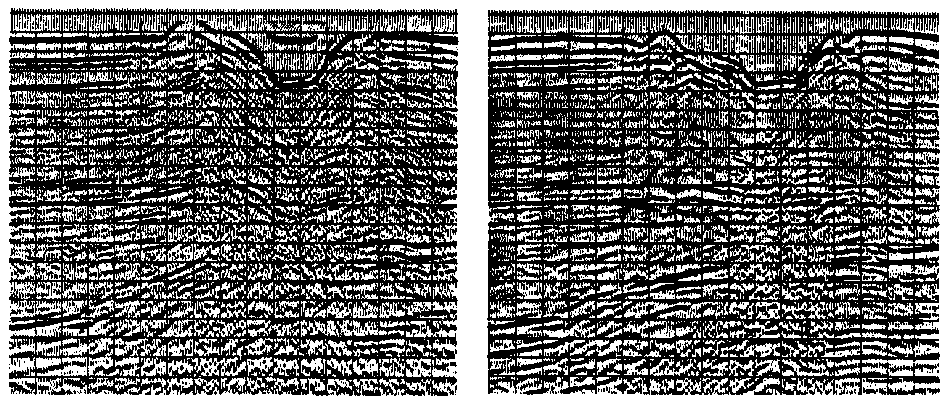
\includegraphics[width=0.65\textwidth]{vdmo/dent}
\caption[dent]{菲律宾地区的资料(左图),经过动态时移校正之后的结果(右图)(据 Dent,1983)}
\label{fig:vdmo/dent}
\end{figure}

\begin{figure}[H]
\centering
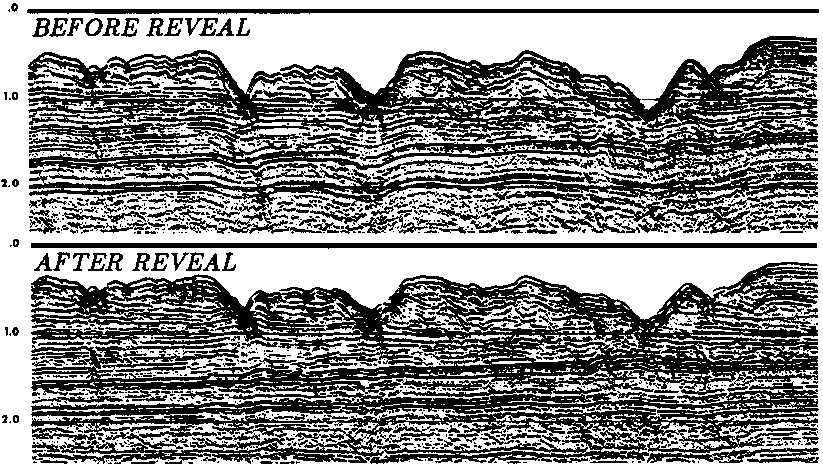
\includegraphics[width=0.65\textwidth]{vdmo/reveal}
\caption[reveal]{采用替代速度进行处理的例子。
可以看出,较深的地层现已较平缓且更连续(Digicon公司提供)}
\label{fig:vdmo/reveal}
\end{figure}

\subsection{双曲线顶点的横向移动}
\label{sec:3.7.2}

图\ref{fig:vdmo/lady}所示是一个点散射体,位于呈三十度倾斜的低速楔形层之下的高速层内,这是许
多横向速度变化问题的一种典型情形。地表上的到达时间将是粗略呈双曲线形,但具有某种畸
变,因为在分界面上出现有速度跳跃变化。时距曲线的极小(即双曲线的顶点)业已偏离它
的通常位置,不是正在该点射散体之上方。可以看出:
\begin{enumerate}
  \item 在极小时间时,射线垂直向上出射;
  \item 极小时间位于该点散射体所在的高速一侧;
  \item 极小时间偏离该散射点的位移,随炮检距之增大而增加。
\end{enumerate}
时距曲线大体呈双曲线形,但是左侧的渐近线给出左侧介质的速度,而右侧的渐近线则给出
右侧介质的速度。

\begin{figure}[H]
\centering
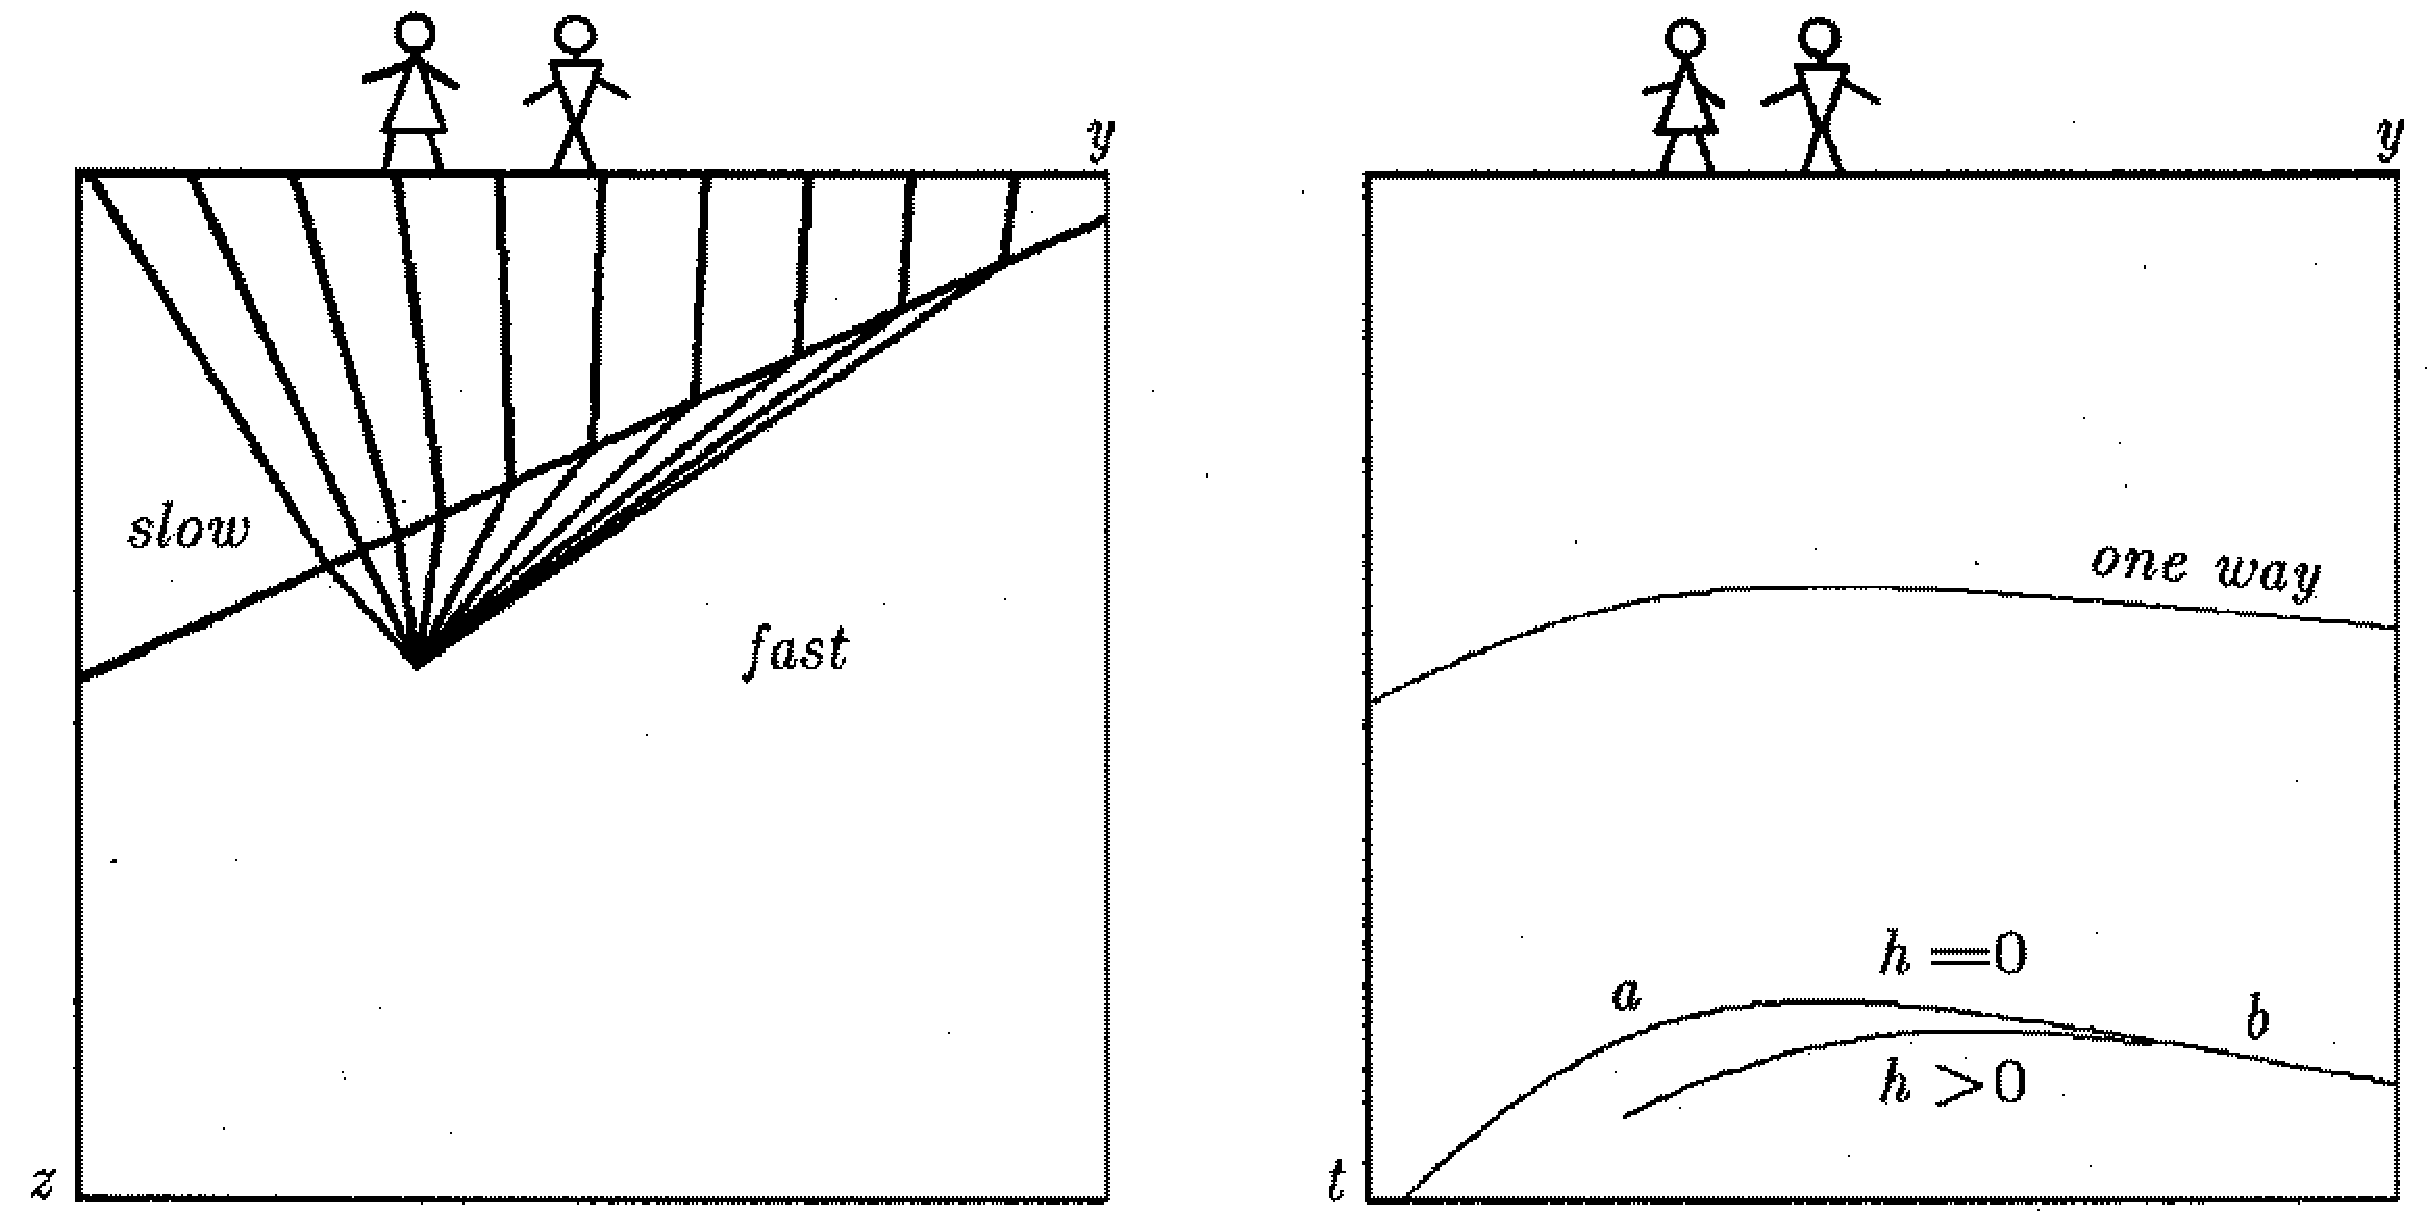
\includegraphics[width=0.65\textwidth]{vdmo/lady}
\caption[lady]{位于速度楔形层之下的散射点的出射线(左图),时距曲线(右图)。
图中,a点处的斜率是b点处斜率之负值。a与b之间的中点位于$h>0$时的曲线之顶部}
\label{fig:vdmo/lady}
\end{figure}

设自散射点至地面$x$点的旅行时间记为$T(x)$,这时对共炮检距剖面来说,旅行时间$t(y)$
就是
\begin{equation*}
t(y)=T(y+h)+T(y-h)
\end{equation*}
为求出最早到达的初至,令$dt/dy=0$,由此可证明图\ref{fig:vdmo/lady}中的$a$点上的斜率应是$b$点上斜率
之负值。这点表明了为什么双曲线顶部偏离散射体的位移是随炮检距而增大的\footnote{
必须同时还考虑到双曲线的不对称性质,才能得此结论。---译者
}。

横向速度变化使双曲线丧失了对称性,从计算上说,这就是透镜项使双曲线发生了歪
斜,引起了它的顶点作横向移动。

\subsection{“幽灵”绕射}
\label{sec:3.7.3}

% 横向速度变化的第二个例子
% 是图\textsuperscript{3}.\textsuperscript{7}-4,该图也是取自Kja-
% rtansson的博士论文。图中所示 物理模型是由代表反射面之断续
% 线段所分开的三个具有恒定速度 的楔形层,该模型的底边也代表l
% 一个反射面•图\textsuperscript{3}.7-4中的波场
% 利用爆炸反射面计算方法作出, Kjartansson把该种计算方法看
% 作是零炮检距剖面的合理近似. 注意,在速度为4公里/秒的楔形
% 层尖端的下方,在底部水平反射 面上有一个小绕射。因为这样一
% 种绕射与可辨认出的平坦反射面 毫无关系,所以给它取名为``幽
% 灵''绕射(Phantom diffract- ion)。幽灵绕射本容易识别,
% 但是它们确实会出现。实际上, 3.1节中所述的``亮点''大概就
% 是幽灵绕射;有人曾报导过,幽 灵绕射为勘探小型的高速灰岩礁
% 提供了一种工具。

% 要利用上表中的倾角关系方程,需知地层倾角$\alpha$,该倾角可由零炮检距剖面测定。在
% Fourier空间内的零炮检距剖面上,该倾角的正弦为$vk_y/2\omega$,其中$k_y$为沿中心点坐标$y$的空
% 间波数;为强调这种测定仅应用于零炮检距剖面,我们总将$\omega$写为$\omega_0$,即
% \begin{equation}
% sin\alpha = \frac{vk_y}{2\omega_0}
% \label{eq:ex3.6.3}
% \end{equation}

% 不存在倾角时,正常时差校正应将任何记录道转换成零炮检距记录道。类似地,存在倾角
% 时,正常时差校正与倾角时差校正联合应用将把任何共炮检距剖面转换为零炮检距剖面。按
% 这种方式由共炮检距剖面制造出来的拟零炮检距剖面(pseudo-zero-offset section)
% 将以$P_0(t_0,h,y)$表示。首先按中心点坐标$y$取其Fourier变换对偶$k_y$,然后遍及时间$t_0$取Four­ier
% 变换,得
% \begin{equation}
% P_0(\omega_0,h,k_y)=\int e^{i\omega_0t_0}P_0(t_0,h,k_y)dt_0
% \label{eq:ex3.6.4}
% \end{equation}
% 将积分变量由$t_0$改变为$t_n$,则
% \begin{equation}
% P_0(\omega_0,h,k_y)=\int \frac{dt_0}{dt_n}e^{i\omega_0t_0(t_n)}P_0(t_0(t_n),h,k_y)dt_0
% \label{eq:ex3.6.5}
% \end{equation}
% 用正常时差校正之后的资料$P_n$来表示被积函数,采用$P_n(t_n,h,k_y)=P_0(t_0(t_n),h,k_y)$的办法即可作到这点
% \begin{equation}
% P_0(\omega_0,h,k_y)=\int \frac{dt_0}{dt_n}e^{i\omega_0t_0(t_n)}P_n(t_n,h,k_y)dt_n
% \label{eq:ex3.6.6}
% \end{equation}
% 同采用Stolt偏移处理时一样,上述变换中与心$dt_0/dt_n$有关的Jacobi函数行列式对各项均起标
% 定作用,但是对时移则不起作用。倾角时差校正(DMO)实际上是利用指数项完成的。

% 略去该Jacobi函数行列式项(它将近为1,作用确实不大),整个处理过程可用程序概
% 略表示如下;
% \begin{minted}{Fortran}
% P(k_y)=FT[P(y)]
% P_n(t_n)=NMO[P(t)]
% for all k_y { #three nested loop, interchangeable
% for all h   { #three nested loop, interchangeable
% for all w_0 { #three nested loop, interchangeable
%         sum=0
%         for all t_n {
%           sum=sum+exp[iw_0[t_n^2+h^2k_y^2/(w_0^2)]^(1/2)]P_n(t_n,h,k_y)
%         }
%         P_0(w_0,h,k_y)=sum
%         }}}
% p_0(t_0,h,y)=FT2D[P_0(w_0,h,k_y)]
% \end{minted}
% 要注意,在程序的内-环中的指数项是与速度无关的.倾角时差校正方程(DMO)中
% 的速度在用式\ref{eq:ex3.6.3}代换$sin\alpha$以后就消失了,所以倾角时差校正并不依赖于速度。

% 以上概述的处理过程要求在倾角时差校正之前进行正常时差校正(NMO)。要是顺序颠
% 倒,就会成为一种近似方法。遗憾的是我们不得不这么颠倒,因为我们不知道速度,宁可在
% 需要进行速度佶计的正常时差校正(NMO)步骤之前来完成计算量大的这种与速度无关之
% 倾角时差校正(DMO))步骤。图\ref{fig:vdmo/dmoproc}为倾角时差校正处理结果。

% \begin{figure}[H]
% \centering
% 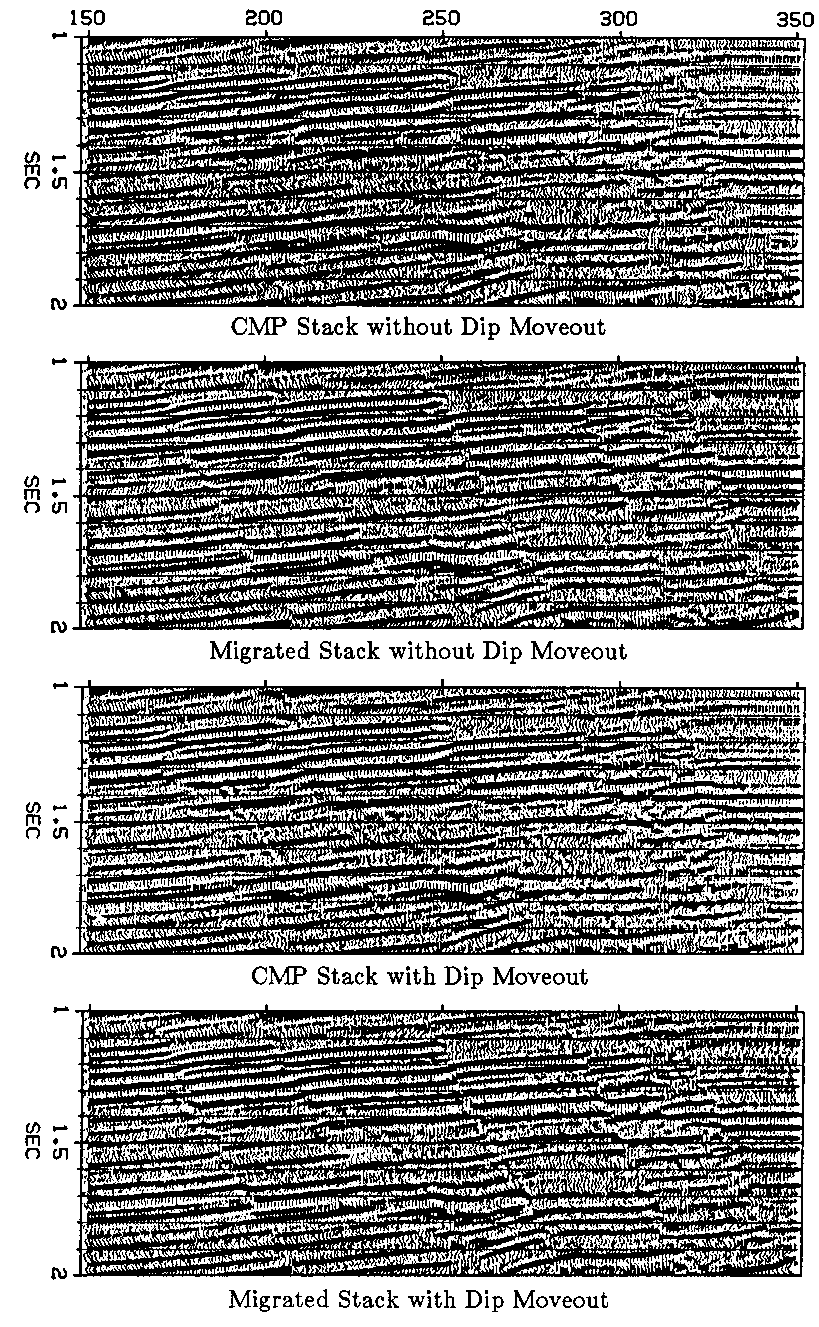
\includegraphics[width=0.65\textwidth]{vdmo/dmoproc}
% \caption[dmoproc]{倾角时差校正处理的剖面(据Hale,1983
% )}
% \label{fig:vdmo/dmoproc}
% \end{figure}

% \subsection{Ottolini 的径向记录道(Radial trace)}
% \label{sec:3.6.4}

% 普通我们都把共中心点道集看作是地震记录道的一个集合,即许多时间函数的集合,
% 每一个时间函数相应于某个特定的炮检距。但是,这种$(h,t)$数据空间能够以不同的坐
% 标系统加以表示。Turhan Taner所介绍的径向记录道系统是具有某些美妙属性的一种坐标
% 系统,在这类系统中,不是按恒定炮检距来取记录道,而是按恒定角度取记录道。这种思
% 想如图\ref{fig:vdmo/otto}所示。

% 除有某些以后将变得更明显的理论优点之外,这种系统还有一些实用优点,其中,值得
% 注意的是:
% (1)各记录道均匀填满非零数据空间;
% (2)在较小时间上,各记录道在短波长之处彼此紧靠近,而在长波长之处则分开较
% 宽;
% (3)给定记录道上的能量代表波动沿一 固定角度方向的传播情况。

% 这最后一个特征对于具有多次反射的数据
% 特别重要(见\ref{sec:5.6}节),不过,就我们的讨论
% 目的而言,径向记录道的最佳属性还是另外一种。

% \begin{figure}[H]
% \centering
% 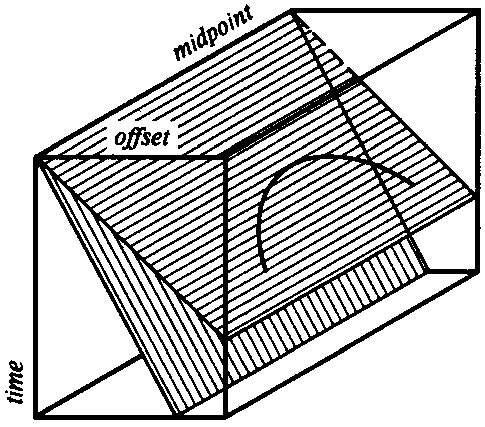
\includegraphics[width=0.65\textwidth]{vdmo/otto}
% \caption[otto]{在反射地震侧线数据体积的内部,是称为径向记录道剖面的平面。
% 地层内部有一个点散射体,则径向记录道剖面上就有一支双曲线}
% \label{fig:vdmo/otto}
% \end{figure}

% Richard Ottolini曾注意到,地层内的
% 点散射体在径向记录道剖面上表现为准确的双
% 曲线,而不是具有平缓顶部的双曲面。点散射
% 体的旅行时间曲线或Cheop金字塔形的曲线
% 族,可写成“弦长度”方程或扁圆方程(见
% \ref{sec:3.2}节)。作下列定义
% \begin{equation}
% sin\phi = \frac{2h}{vt}
% \label{eq:ex3.6.7}
% \end{equation}
% 并代入\ref{sec:3.2}节中的式\ref{eq:ex3.2.13}内,得
% \begin{equation}
% vt=2[\frac{z^2}{cos^2\phi}+(y-y_0)^2]^{1/2}
% \label{eq:ex3.6.8}
% \end{equation}
% 用$cos\phi$来标定$z$轴,又完全重现圆和双曲线的情形!现将隐含的双曲緣表示成图\ref{fig:vdmo/ottohyp}中所
% 示的三维图像。

% \begin{figure}[H]
% \centering
% 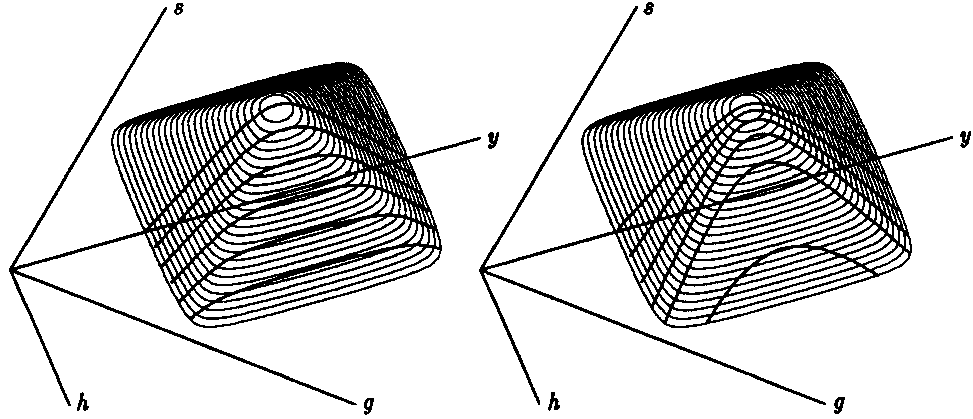
\includegraphics[width=0.65\textwidth]{vdmo/ottohyp}
% \caption[ottohyp]{在Cheop金字塔中是平顶的双曲线,在径向记录道剖面上却是绕射双曲线}
% \label{fig:vdmo/ottohyp}
% \end{figure}

% 我们将会看到,图\ref{fig:vdmo/ottohyp}中的径向剖面内的双曲线比固定炮检距$h$时所看到的平顶双曲
% 面更容易掌握一些。参考下表定义倾角时差校正的方程和定义径向记录道坐标系内之普通的
% 时差校正的方程,就会明白这点。

% 下表中的第二个方裎就是零炮检距偏移采用的爆炸反射面方程,在双平方根方程中令
% $H=0$也可以得出该式。如该式所示,它包含有地层速度而不是半速。方程\ref{eq:ex3.6.8}说明,用
% $cos\phi$将$z$坐标轴加以标定,则不同分值时的各双曲线就全都联系在一起,具有同一个形式了。
% 根据Fourier变换理论,用一个除因子$cos\phi$对$z$进行标定就会相当于甩一个乘因子$cos\phi$将$k_z$
% 加以标定。这就意味着,上表第一个方程可以适用于径向记录道剖面上的偏移双曲线和绕射
% 双曲线\footnote{
% 这个方程即是径向记录道剖面信移与统射的频散方程,炮检距信息隐藏于角度参量命内。---译者}。
% 从第一个和第二个方程中消去$k_z$,得出上述$\omega\rightarrow\omega_0$时的第三个方程,这个方程把
% 所有炮检距(实际上就是任何径向角度)偏移至零炮检距的运算同后来在零炮检剖面上进行
% 绕射扫描的运算全结合在一起了,所以总效果就是炮检距延拓、即正常时差校正(NMO)
% 和倾角时差校正\footnote{
% 这个频散方程所描述的是将径向剖面转换为零炮检距平面的运箅过程,它将$\omega$转换为$\omega_0$,事实上就是将时间$t$转
% 换为中心点位置上的双程垂直时间$t_0$。---译者
% }(DMO)。上表最后两个方程是把$\omega\rightarrow\omega_0$时的第三个方程分解成$\omega\rightarrow\omega_s$和
% $\omega_s\rightarrow\omega_0$的两个相继过程,这两个处理过程像是DMO和NMO,但是运算均在径向空间内进
% 行。径向NMO是一种简单的时不变(time-invariant)拉伸,因此采用符号$\omega_s$。

% 同共炮检距剖面的情形不同,现在的径向空间之倾角时差校正是能够在进行拉伸、速度
% 估计这些步骤之前完成的。让我们来论证一下倾角时差校正确实真的与速度无关。将式\ref{eq:ex3.6.7}代入前述表格中的径向DMO变换,得到由时间$t$至拉伸时间的变换方程
% \begin{equation}
% \frac{h^2}{t^2}k_y^2+\omega_s^2=\omega^2
% \label{eq:ex3.6.9}
% \end{equation}
% 我们可观察到速度$v$已经在式\ref{eq:ex3.6.9}中消失掉了,所以径向坐标系中的倾角时差校正确实
% 不依赖于速度,进行倾角时差校正的处理$\omega\rightarrow\omega_s$并不要求有速度信息。径向坐标系提供的好
% 处就是这种计算量相当大的处理可以在进行速度估计$\omega_s\rightarrow\omega_0$之前来完成。

% 利用式\ref{eq:ex3.6.9},倾角时差校正过程$\omega\rightarrow\omega_s$可以很方便地采用一种Stolt型的算法来实现。

% 前面的分析均已假设速度为常数。在倾角时差校正之后,即将进行常规速度分析、叠加
% 和零炮检距偏移之前,可以采用有效的实用近似方法恢复为对速度$v(z)$随深度而变情形的分
% 析。

% 无论径向记录道方法还是Hale的共炮检距方法都能在恒定速度介质中准确地解决所有
% 角度问题,可是没有一种方法能准确处理速度分层情形下的问题,连能否作到这点也不清楚
% ---因为没有一种方法是源于双平方根方程的。Yilmaz(1979)关于DMO方面的工作是源
% 于双平方根方程的。所以他的方法对于速度分层情形可望是严格的,但是Yilmaz也不能避
% 免与角度有关的近似处理问题。因此,理论工作尚有待完成。

% \subsection{倾角时差校正的抗假频特性}
% \label{sec:3.6.5}

% 你可能会想,如果将空间$(y,h,t)$以采样间隔$\Delta y$沿$y$轴采样,则任何最终偏移剖面
% $P(y,z)$将没有比$\Delta y$更高的空间分辨率了。其实情形并不这样。

% 此处起作用的基本原理自Shannon时代以来就已经知道了,如果一个时间函数及其导数
% 均按时间间隔$2\Delta t$进行采样,倘若信号的原始宽度低于$1/(2\Delta t)$,则它们就可以完全重
% 建。更一般性地说,如果一个信号用m个独立的滤波器来滤波,而且所得这m个信号均按间
% 隔来采样,则该信号就可以被恢复。

% 这里的问题是如何将这种概念应用于地震资料。基本信号是地层模型,它的各种不同滤
% 波后的形式就是共炮检距剖面。记住,当增大炮检距时,CDP叠加的反射点是移向上倾方向
% 的。进一步的细节可参阅Bolondi、Loinger和Rocca(1982)的论文,他们首次指出了倾角
% 时差校正的抗假频特性。在对三维地震资料的兴趣日益增大的这个时期,应该对倾角时差校
% 正的抗假频的特性给予特别的注意。




% \subsection{习题}
% \label{sec:3.6.6}

% \begin{enumerate}
% \item 试述Hale的倾角时差校正处理中Jacobi函数行列式的影响。

% \end{enumerate}
